\section{Appendix}
\subsection{Class diagram}
Text

\newpage
\subsection{Statechart diagram}
Text

\newpage
\subsection{Alloy}
\subsubsection{Purpose}
% EDO: per me questa sezione si potrebbe eliminare
% LKPC: per me si potrebbe aggiungere una breve motivazione che spieghi quali componenti abbiamo preferito mdoellare in alloy e perch�, tipo: "Abbiamo modellato in alloy i componenti che riteniamo necessitino di una verifica formale atta a garantire la correttezza delle specifiche relativamente alle operazioni service-critical caratterizzanti la piattaforma PowerEnJoy (che detta in parole povere: voglio essere sicuro che la specifica non consenta a chiunque di fottersi le macchinette...).
Following are some Alloy models for system components that we believe require a formal checking apt to ensure specifications correctness with respect to service-critical operations characterizing the PowerEnJoy platform.
\subsubsection{Code}
\begin{itemize}
\item Reserved Cars Unlocking 

\lstinputlisting[language=alloy]{Alloy_code/unlockCars_v2.als}


5 commands were executed. The results are:\newline
   -1: Instace found.unlockCar is consistent.\newline
   -2: No counterexample found. TwoCarAreSame may be valid.\newline
   -3: No counterexample found. NoUserUnlockBookedCar may be valid.\newline
   -4: No counterexample found. NoMultipleCarWithSameID may be valid.\newline
   -5: No counterexample found. UserMakeRequest may be valid.
   
\newpage

\item Unlocking Cars World
\newline
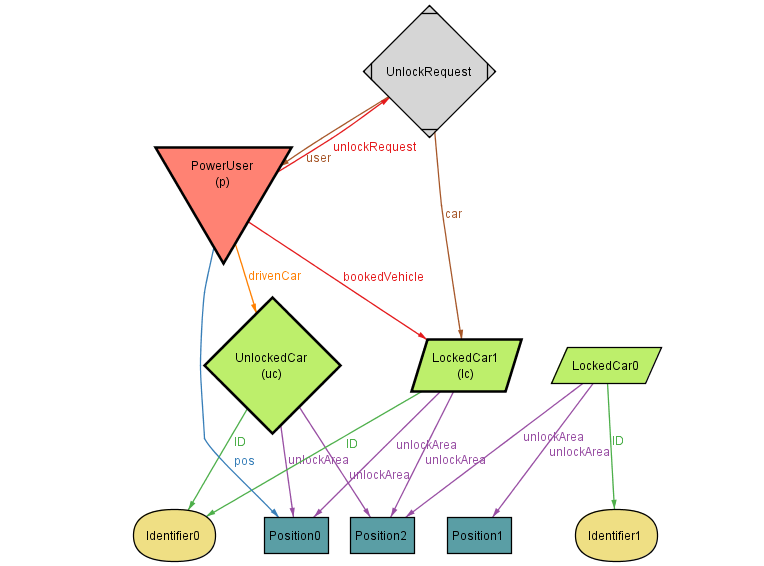
\includegraphics[scale=0.5]{{Alloy_code/unlockCar_world.png}}


\item  Cars Lock
   
   
\end{itemize}   

\subsubsection{Example worlds}
Text